\documentclass[tikz,border=8pt]{standalone}
% Shared look for every TikZ diagram. Load with \input{../../tools/tikz-style.tex}
\usepackage[T1]{fontenc}
\usepackage{lmodern}
\renewcommand{\sfdefault}{lmr}  % diagrams use the same serif as the text
\usetikzlibrary{arrows.meta, positioning, shapes.geometric, calc, fit, backgrounds}
\definecolor{cblue}{HTML}{4C78A8}
\definecolor{corange}{HTML}{F58518}
\definecolor{cgreen}{HTML}{54A24B}
\definecolor{cred}{HTML}{E45756}
\definecolor{cpurple}{HTML}{B279A2}
\definecolor{cgrey}{HTML}{6B6B6B}
\tikzset{
  every picture/.style={font=\sffamily, line width=1.2pt},
  box/.style={draw=#1, fill=#1!12, rounded corners=4pt, align=center, inner sep=7pt, minimum height=1.1cm},
  box/.default=cgrey,
  arrow/.style={-{Stealth[length=3mm]}, draw=cgrey, line width=1.4pt},
  title/.style={font=\sffamily\bfseries\Large},
  note/.style={font=\sffamily\small, text=cgrey, align=center},
}
\AtBeginDocument{\hyphenpenalty=10000 \exhyphenpenalty=10000}

\begin{document}
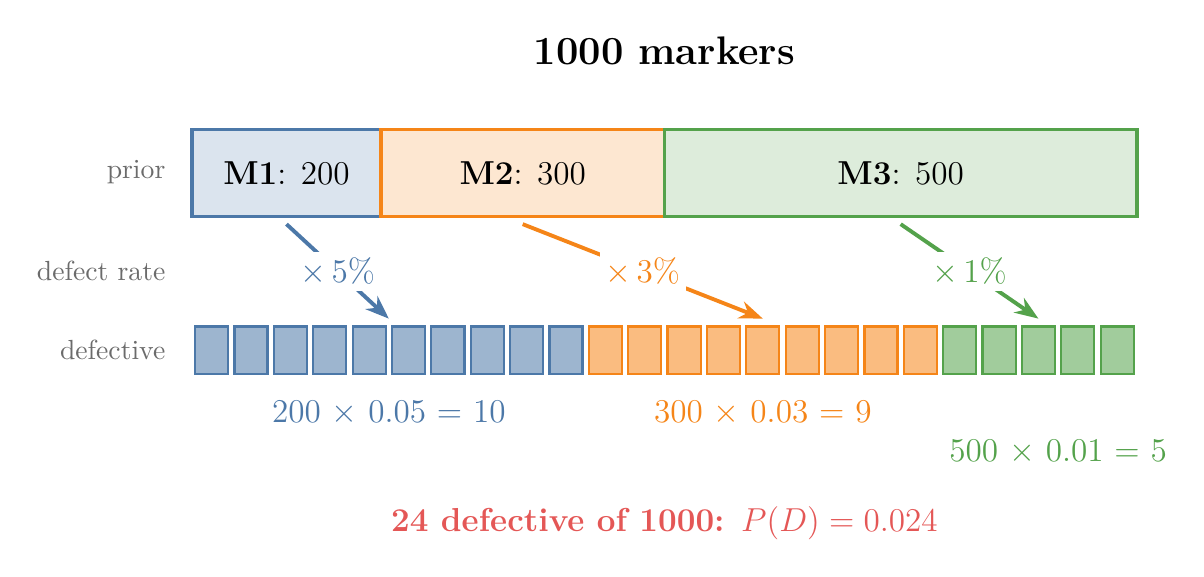
\begin{tikzpicture}[every node/.append style={font=\sffamily\large}]
  % top bar: 1000 markers, widths to scale (12 cm = 1000)
  \node[title] at (6,2.1) {1000 markers};
  \foreach \x/\w/\c/\m/\n in {0/2.4/cblue/M1/200, 2.4/3.6/corange/M2/300, 6/6/cgreen/M3/500} {
    \draw[draw=\c, fill=\c!20, line width=1.2pt] (\x,0) rectangle ++(\w,1.1);
    \node at (\x+\w/2,0.55) {\textbf{\m}: \n};
  }
  \node[note, anchor=east, font=\sffamily] at (-0.2,0.55) {prior};
  % likelihood labels: arrows land on each machine's group of defective squares
  \foreach \cx/\gx/\c/\r in {1.2/2.5/cblue/5\%, 4.2/7.25/corange/3\%, 9/10.75/cgreen/1\%} {
    \draw[arrow, draw=\c] (\cx,-0.1) -- (\gx,-1.3) node[midway, text=\c, fill=white, inner sep=2pt] {$\times$\,\r};
  }
  \node[note, anchor=east, font=\sffamily] at (-0.2,-0.7) {defect rate};
  % bottom row: 24 defective markers, 0.5 cm each
  \foreach \i in {0,...,23} {
    \ifnum\i<10 \def\c{cblue}\else\ifnum\i<19 \def\c{corange}\else\def\c{cgreen}\fi\fi
    \draw[draw=\c, fill=\c!55, line width=0.8pt] (0.5*\i+0.04,-2.0) rectangle ++(0.42,0.6);
  }
  \node[text=cblue] at (2.5,-2.5) {200 $\times$ 0.05 = 10};
  \node[text=corange] at (7.25,-2.5) {300 $\times$ 0.03 = 9};
  \node[text=cgreen] at (11.0,-3.0) {500 $\times$ 0.01 = 5};
  \node[note, anchor=east, font=\sffamily] at (-0.2,-1.7) {defective};
  \node[font=\sffamily\large\bfseries, text=cred] at (6,-3.9) {24 defective of 1000: $P(D) = 0.024$};
\end{tikzpicture}
\end{document}
